\documentclass[hidelinks,12pts]{article}
\usepackage[export]{adjustbox}
\usepackage{amsmath}
\usepackage{amssymb}
\usepackage[title,titletoc]{appendix}
\usepackage{array}
\usepackage[english]{babel}
\usepackage{bbm}
\usepackage{blindtext}
\usepackage{bookmark}
\usepackage{booktabs}
\usepackage{cancel}
\usepackage{caption}
\usepackage{csquotes}
\usepackage{enumerate}
\usepackage{enumitem}
\usepackage{epigraph}
\usepackage[left]{eurosym}
\usepackage{float}
\usepackage[bottom]{footmisc}
\usepackage[margin=0.9in]{geometry}
\usepackage{graphicx}
\usepackage{hyperref}
\usepackage{indentfirst}
\usepackage{lscape}
\usepackage{mathtools}
\usepackage{mdframed}
\usepackage{multirow}
\usepackage{multicol}
\usepackage[sort]{natbib}
\usepackage{parskip}
\usepackage{setspace}
\usepackage{subcaption}
\usepackage{titlesec}
\usepackage{tgpagella}
\usepackage{varwidth}
\usepackage{verbatim} %comment block
\usepackage{wrapfig}
\usepackage[dvipsnames]{xcolor}
\usepackage{xltabular}

\renewcommand{\epigraphsize}{\normalsize}
\setlength{\epigraphwidth}{0.7\textwidth}
\renewcommand{\textflush}{flushright}
\renewcommand{\sourceflush}{flushright}


\renewcommand\appendixpagename{Mathematical Appendix}
\renewcommand{\baselinestretch}{1.45}

\hypersetup{
    colorlinks=true, 
    urlcolor= Violet, 
    linkcolor=Black, 
    citecolor=Blue, 
    filecolor = Blue
    } 

%\usepackage{natbib}
\bibliographystyle{plainnat}
%\bibdata{My Library.bib}
%\usepackage[backend=biber, style=authoryear-icomp]{biblatex}

\DeclareMathOperator{\E}{\mathbb{E}}
\DeclareMathOperator{\Prb}{\mathbb{P}}
\DeclareMathOperator{\R}{\mathbb{R}}
\DeclareMathOperator{\N}{\mathbb{N}}
\DeclareMathOperator{\1}{\mathbbm{1}}
\newcommand{\ind}{\perp\!\!\!\!\perp}


\titleformat{\part}{\centering\normalfont\Large\bfseries}{\partname\hspace{5pt}\thepart\hspace{5pt}}{5pt}{--\ }

\titleformat{\part}{\centering\normalfont\Large\bfseries}{\partname\hspace{5pt}\thepart\hspace{5pt}}{5pt}{--\ }

\makeatletter
\def\@fnsymbol#1{\ensuremath{\ifcase#1\or \dagger\or \ddagger\or
   \mathsection\or \mathparagraph\or \|\or **\or \dagger\dagger
   \or \ddagger\ddagger \else\@ctrerr\fi}}
    \makeatother


\begin{document}

        \title{\scshape{Financial Econometrics 1 - M2 FTD \\ Empirical Applications}}
        \author{Luis Miguel Fonseca \\ Stéphane Eloundou Mvondo\\ Natalia Cárdenas Frías }
        \date{\today}
        \maketitle 

\tableofcontents
\newpage


\section*{Introduction} \addcontentsline{toc}{section}{\protect\numberline{}Introduction}
\textcolor{blue}{something, probably describe how all applications make sense one after the other and what is the research question we could have made ourselves when doing the applications, try to give a coherent look to the whole thing.}

This document compiles all our applications of the Financial Econometrics course. 
Each section represents a specific application, but we tried to make them coherent across them around a broad question: 





\section{Series Dynamics}\label{sec:dynamics}

\textcolor{gray}{\emph{Note:} Depending on each exercise along these applications we might use different series. In this first section, we performed the stationarity and component analysis of all of them to be able to use them rapidly without having to worry about seasonality or the presence of UR. Therefore, this section encompasses more than the 3 series that were asked in the exercise.}

\begin{figure}[h!]
    \centering
    \begin{subfigure}[b]{0.8\textwidth}
        \centering
        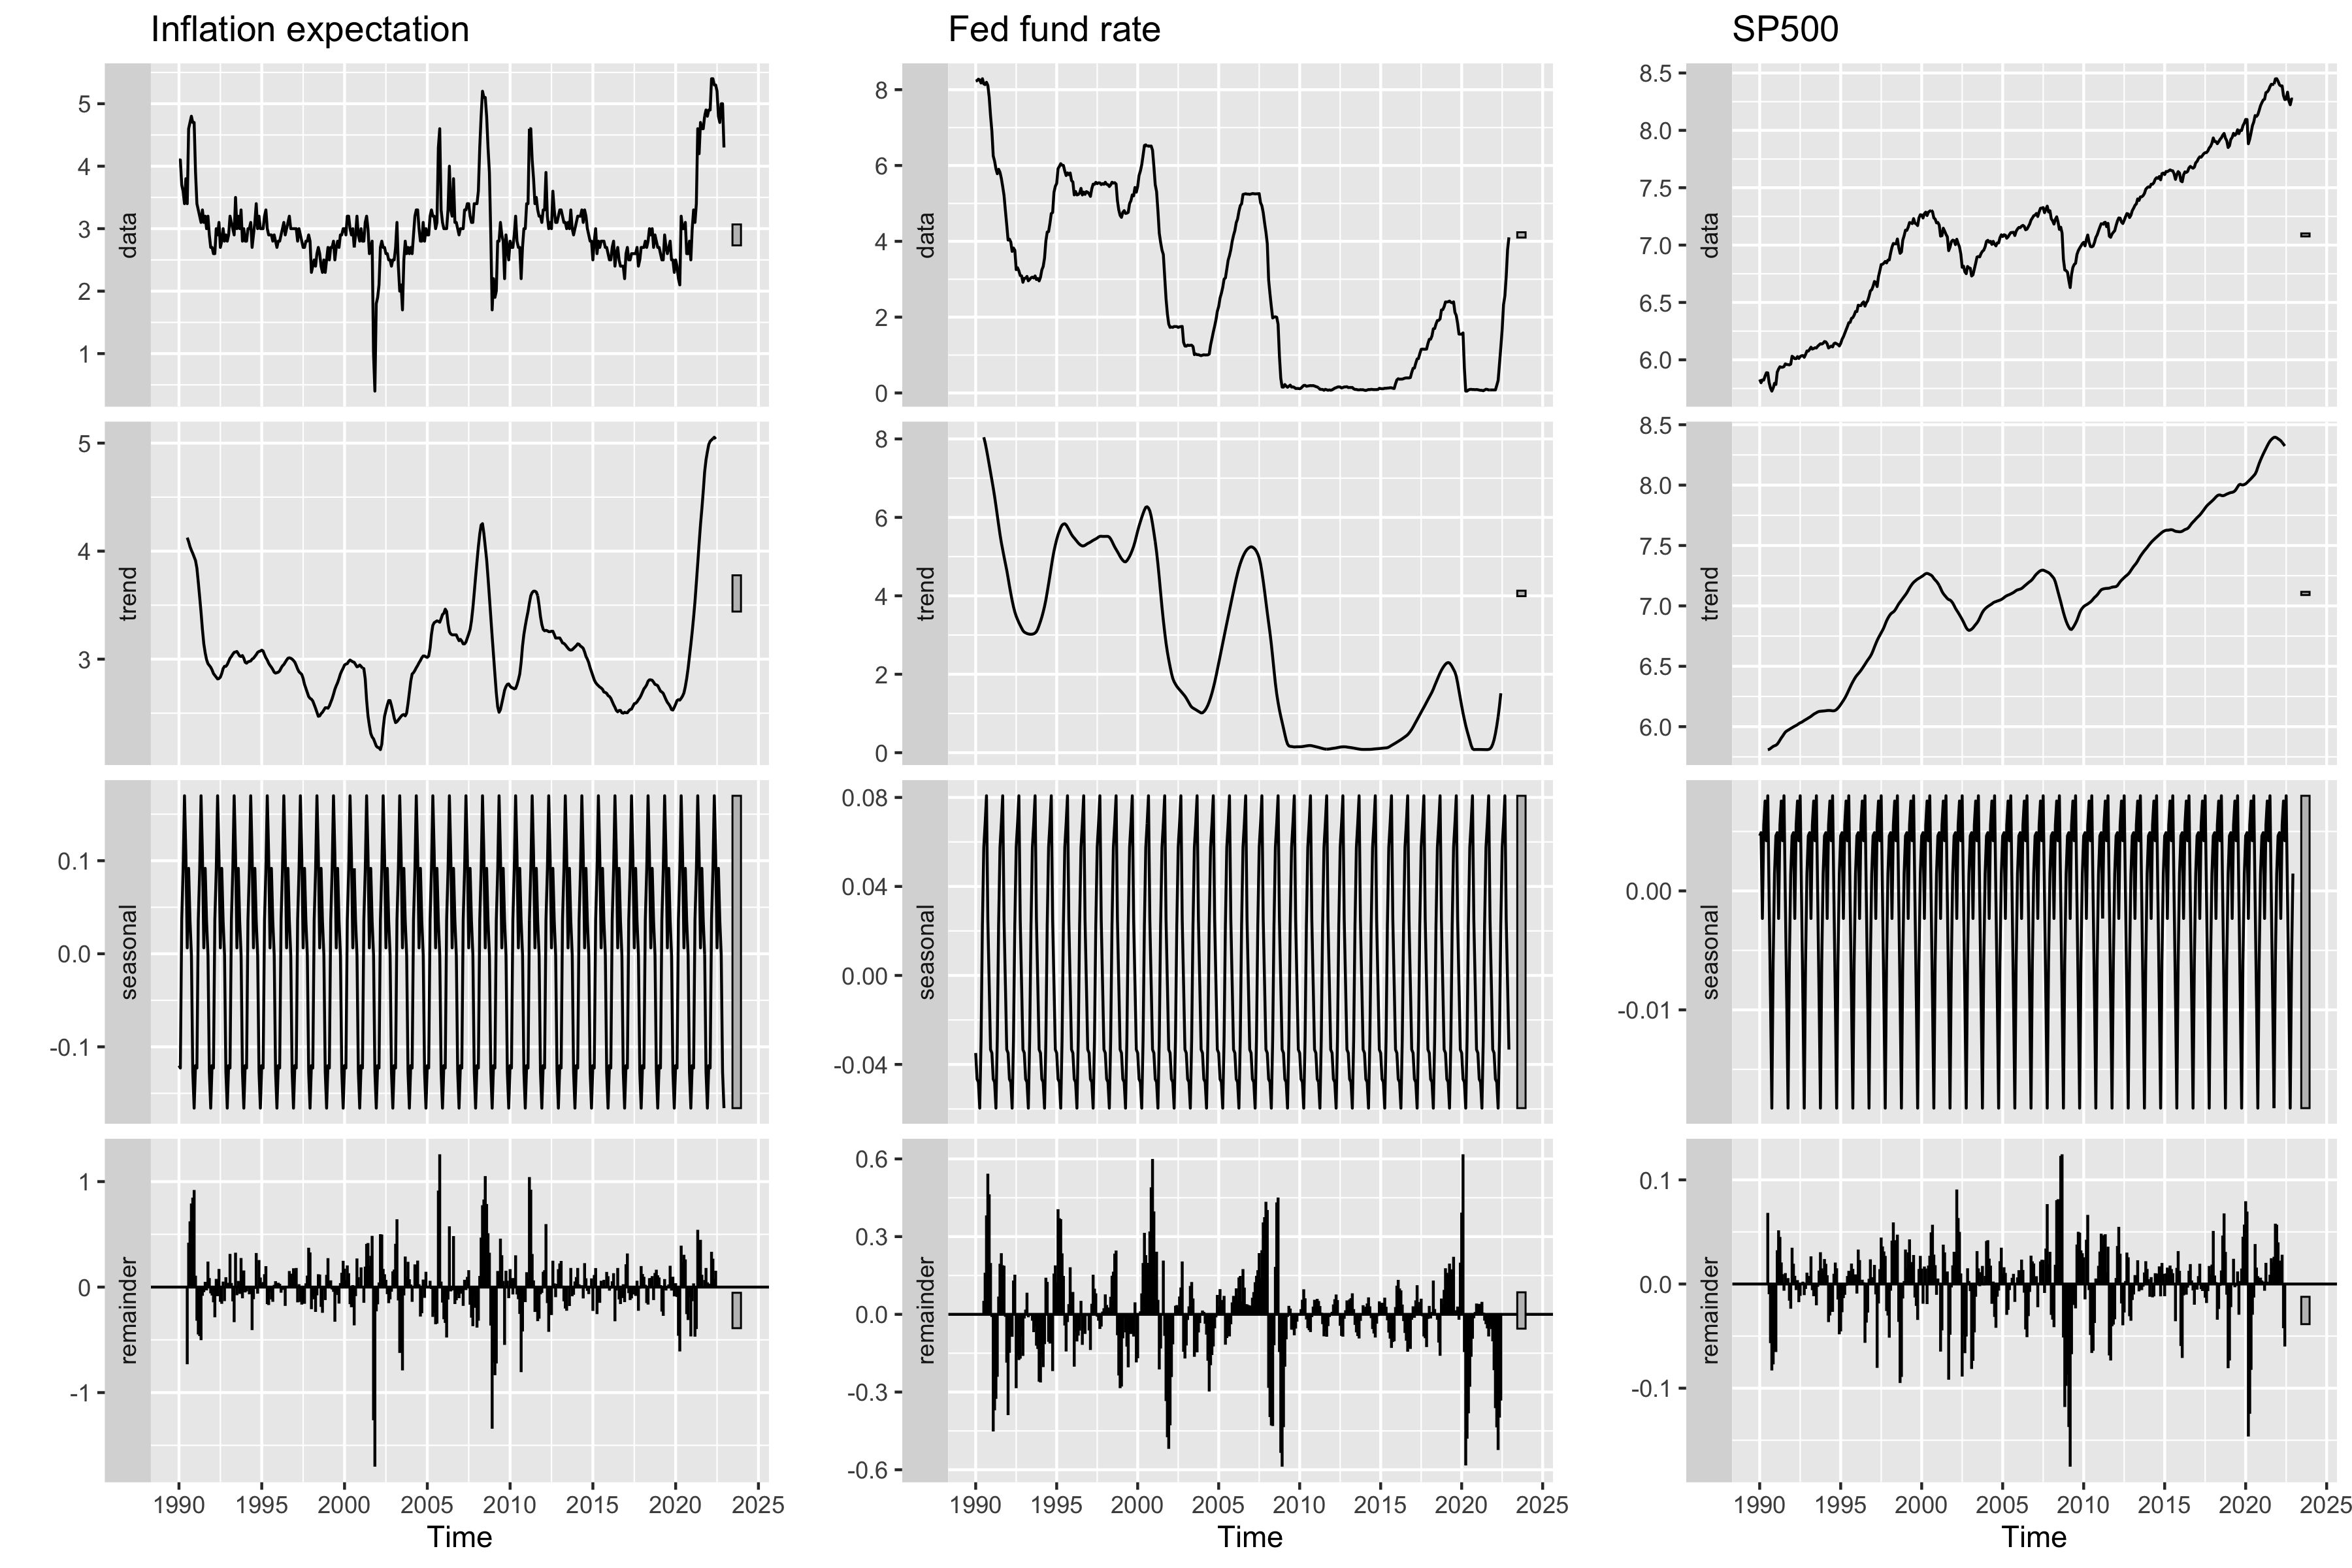
\includegraphics[width=\textwidth]{IMAGES/decomposition_i.png}
        \caption*{}
    \end{subfigure}
    \hfill
    \begin{subfigure}[b]{0.8\textwidth}
        \centering
        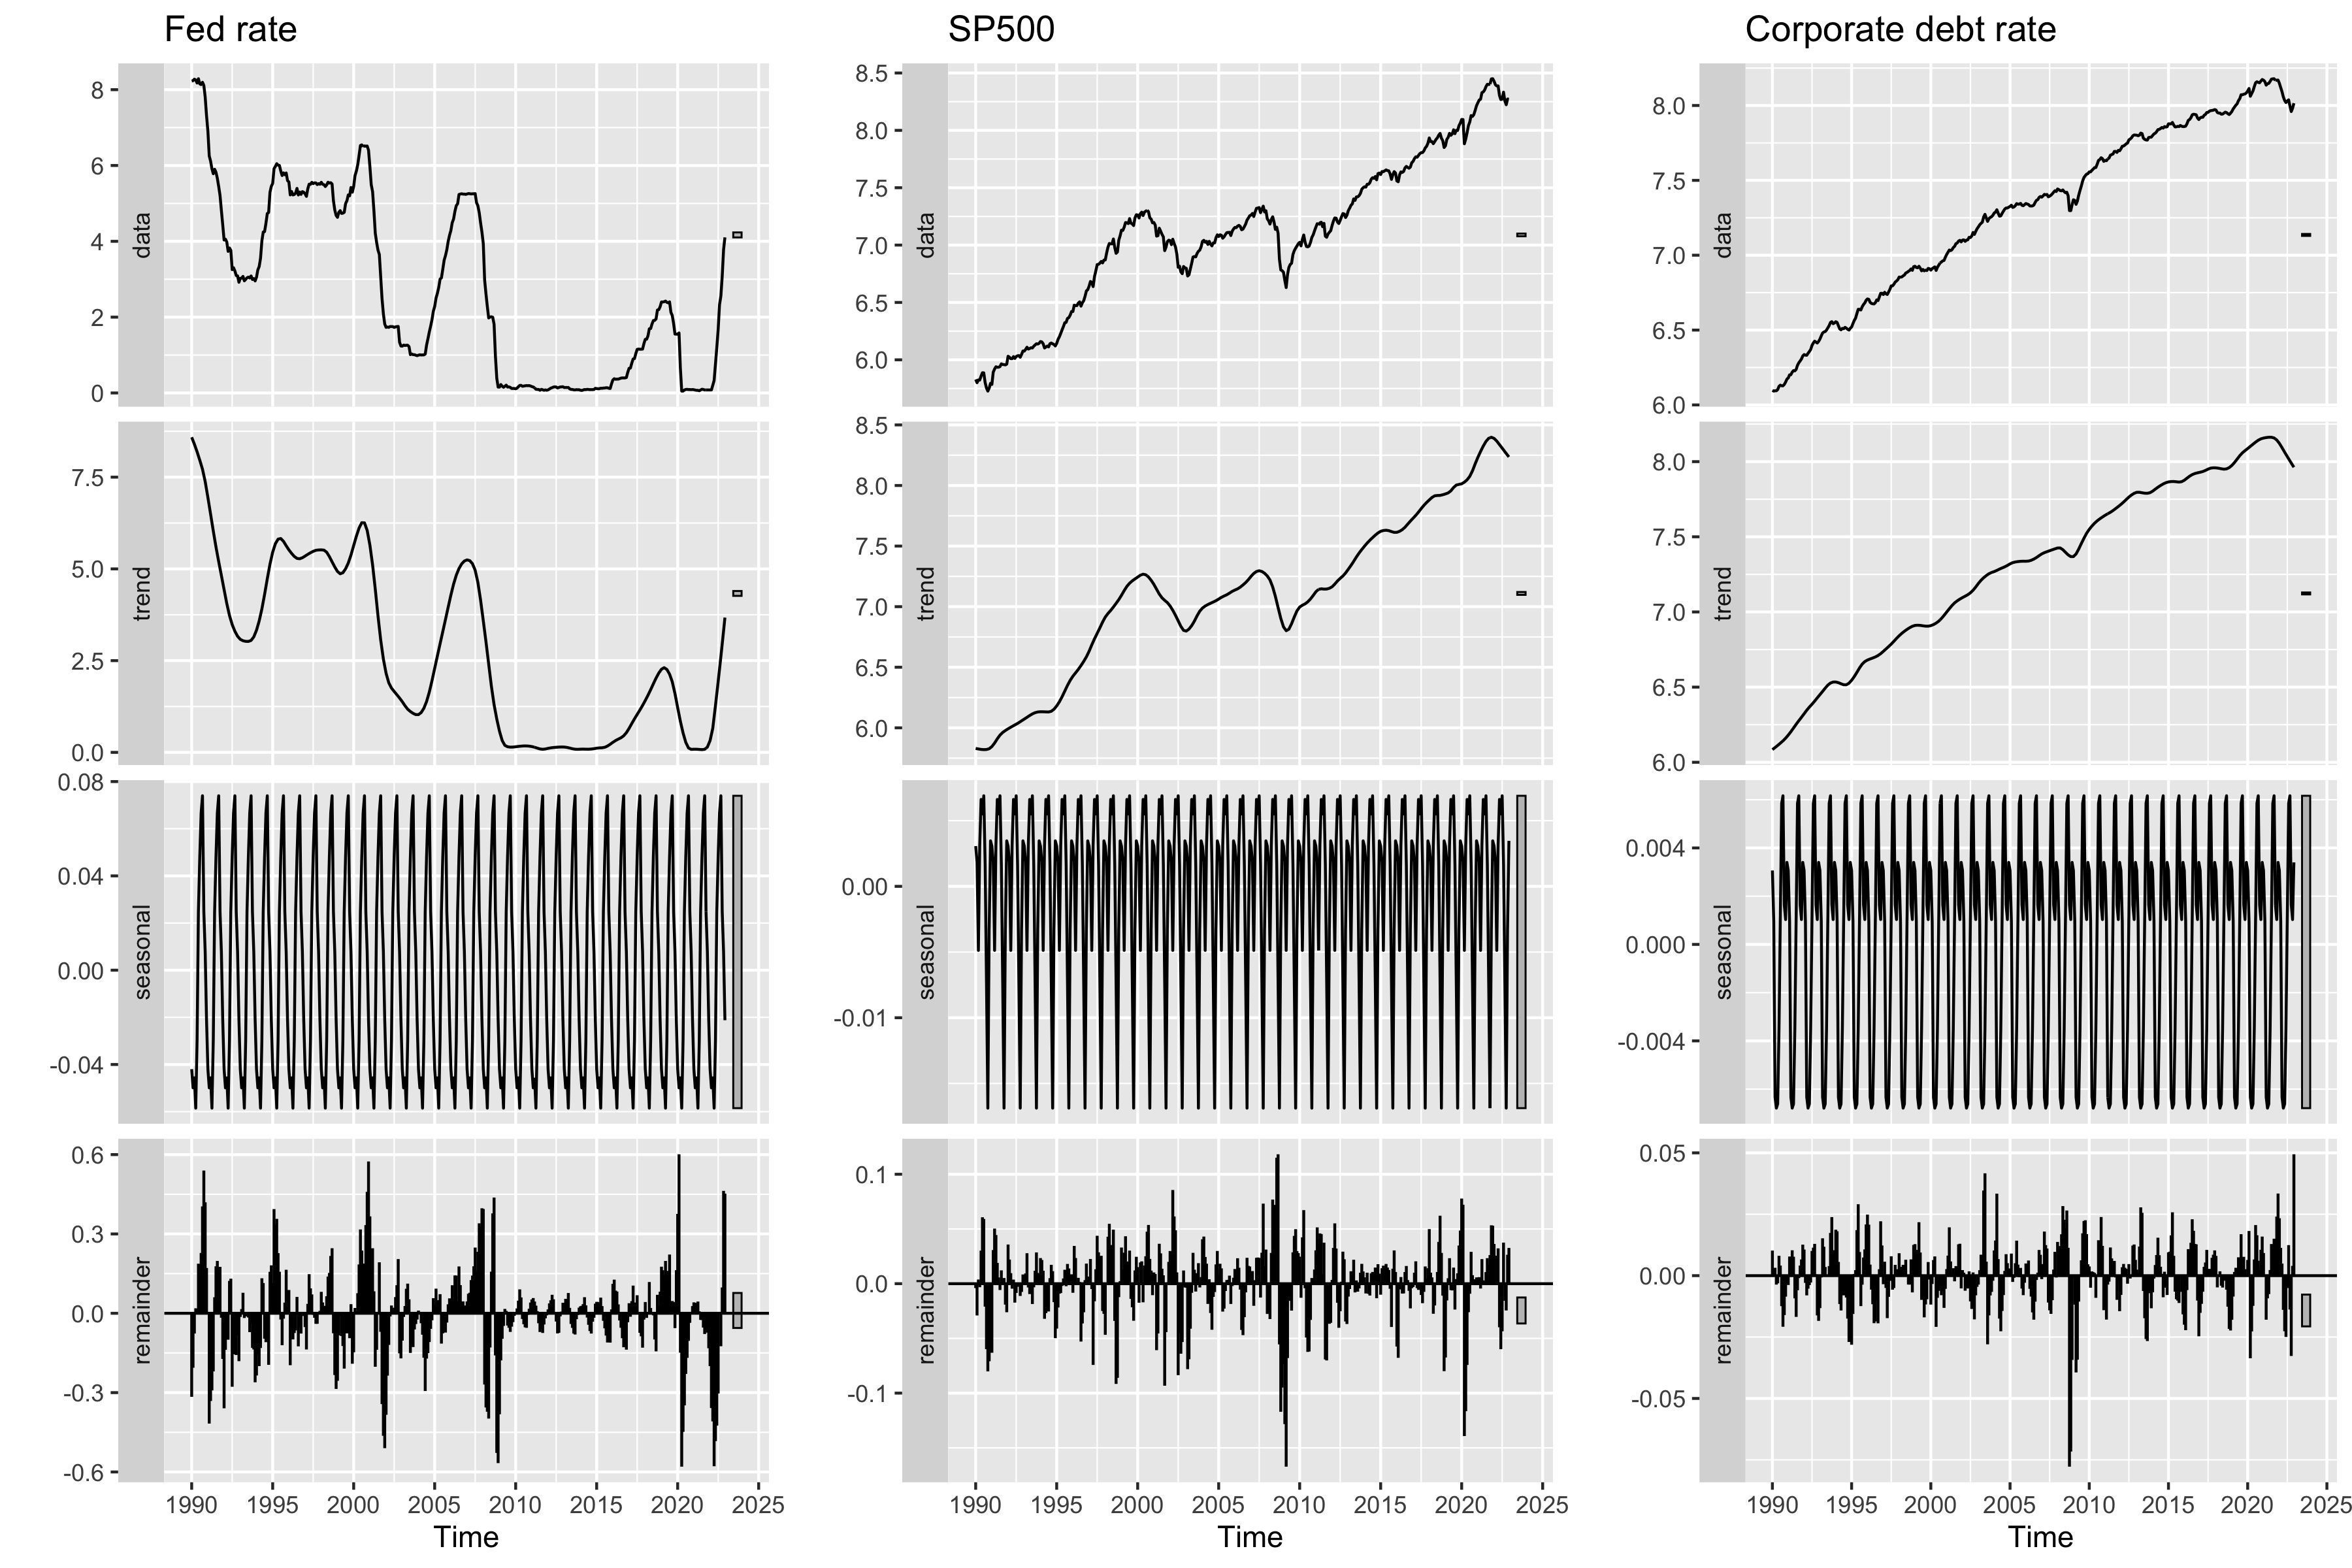
\includegraphics[width=\textwidth]{IMAGES/decomposition_ii.png}
        \caption*{}
    \end{subfigure}
    \hfill 
    \caption{Time series decomposition}
    \label{fig:decomposition}
\end{figure}

    \subsection{Seasonality}

% Table created by stargazer v.5.2.3 by Marek Hlavac, Social Policy Institute. E-mail: marek.hlavac at gmail.com
% Date and time: Tue, Dec 05, 2023 - 20:24:19
\begin{table}[!htbp] \centering 
  \caption{Estimation of the seasonality of each series} 
  \label{tab:seasons} 
\begin{tabular}{@{\extracolsep{5pt}} ccccccccccccc} 
\\[-1.8ex]\hline 
\hline \\[-1.8ex] 
 & JAN & FEB & MAR & APR & MAY & JUN & JUL & AUG & SEP & OCT & NOV & DEC \\ 
\hline \\[-1.8ex] 
infl\_e & -0.104 & -0.108 & 0.031 & 0.078 & 0.149 & 0.1 & 0.017 & 0.088 & 0.031 & 0.006 & -0.116 & -0.173 \\ 
deflator & 0.018 & 0.035 & 0.053 & 0.072 & 0.06 & 0.045 & 0.03 & -0.024 & -0.078 & -0.128 & -0.072 & -0.012 \\ 
unempl & 0.464 & 0.327 & 0.132 & -0.045 & -0.074 & 0.296 & 0.284 & 0.007 & -0.257 & -0.406 & -0.379 & -0.349 \\ 
rate & -0.042 & -0.05 & -0.046 & -0.059 & -0.03 & 0.025 & 0.048 & 0.067 & 0.074 & 0.025 & 0.008 & -0.021 \\ 
splong & 0.003 & 0.002 & -0.005 & 0.003 & 0.007 & 0.006 & 0.007 & 0.002 & -0.007 & -0.017 & -0.003 & 0.003 \\ 
corp\_debt & 0.003 & 0.001 & -0.006 & -0.007 & -0.007 & -0.004 & 0.001 & 0.006 & 0.006 & 0.002 & 0.001 & 0.003 \\ 
\hline \\[-1.8ex] 
\end{tabular} 
\end{table} 


    \subsection{Unit root and trends}

\paragraph*{ADF - Test jointly for deterministic and stochastic trend (with drift)}

We first run the following specification to the ADF model to \emph{jointly} investigate the presence of a stochastic and a determinist trend for each series $(X_t)_t$: 
    \begin{equation}
        \Delta X_t = \alpha + \beta tt + \gamma X_{t-1} +\sum_{i=1,2,..}\rho_i \Delta X_{t-i} + \varepsilon_t
    \end{equation}
As per usual, the ADF test assumes H0: $\gamma =0$ i.e. a unit exists and the series is non-stationary. 
We use R's built in function \emph{ur.df} with \emph{type='trend'} to get this estimation. 

Let us examine each series' results: 
\begin{itemize}
    \item  Inflation expectation,% $t_\gamma = -4.490 < -3.43$ \footnote{Remark that the critical value in both tables can be a little different. This is because they are sensitive to the number of observations in each series. In Table \ref{tab:adftrend_hyp}, the critical values correspond to those provided directly by R and are associated to $N=500$, while in Table \ref{tab:tstat_trend} we give the values for $N=250$. Since we have 396 data points per series we prefer to refer to the higher critical values but it does not change the analysis done.} we can reject HO ie we can't say that the series has a UR. To be sure of this conclusion we compare the t-statistics associated to $\alpha$ and $\beta$ to the standard $-1.96$ threshold 
    \item Fed fund rate, $t_\gamma = -1.709$
\end{itemize}





% Table created by stargazer v.5.2.3 by Marek Hlavac, Social Policy Institute. E-mail: marek.hlavac at gmail.com
% Date and time: Mon, Dec 11, 2023 - 11:28:39
\begin{table}[!htbp] \centering 
  \caption{ADF test - 1st regression with drift, deterministic trend and stochastic trend} 
  \label{tab:adftrend_hyp} 
\begin{tabular}{@{\extracolsep{5pt}} cccccccccc} 
\\[-1.8ex]\hline 
\hline \\[-1.8ex] 
 & infl\_e & deflator & unempl & rate & splong & corp\_debt & CV 1pct & CV 5pct & CV 10pct \\ 
\hline \\[-1.8ex] 
tau3 & $$-$4.650$ & $$-$5.197$ & $$-$3.763$ & $$-$1.709$ & $$-$1.975$ & $$-$1.867$ & $$-$3.980$ & $$-$3.420$ & $$-$3.130$ \\ 
phi2 & $7.375$ & $9.097$ & $4.769$ & $2.015$ & $3.875$ & $10.326$ & $6.150$ & $4.710$ & $4.050$ \\ 
phi3 & $11.061$ & $13.644$ & $7.134$ & $2.917$ & $1.997$ & $4.247$ & $8.340$ & $6.300$ & $5.360$ \\ 
\hline \\[-1.8ex] 
\end{tabular} 
\end{table} 

%
% Table created by stargazer v.5.2.3 by Marek Hlavac, Social Policy Institute. E-mail: marek.hlavac at gmail.com
% Date and time: Sun, Dec 03, 2023 - 17:49:05
\begin{table}[!htbp] \centering 
  \caption{ADF test - 1st regression with deterministic and stochastic trend} 
  \label{} 
\begin{tabular}{@{\extracolsep{5pt}} ccccccc} 
\\[-1.8ex]\hline 
\hline \\[-1.8ex] 
 & Series & Estimate & Std. Error & t value & Pr(\textgreater \textbar t\textbar ) & Fstat \\ 
\hline \\[-1.8ex] 
X.Intercept. & infl\_e & $0.310$ & $0.080$ & $4$ & $0$ & $8.050$ \\ 
z.lag.1 & infl\_e & $$-$0.110$ & $0.020$ & $$-$4.650$ & $0$ & $3$ \\ 
tt & infl\_e & $0$ & $0$ & $1.270$ & $0.210$ & $390$ \\ 
z.diff.lag & infl\_e & $$-$0.010$ & $0.050$ & $$-$0.250$ & $0.800$ & $8.050$ \\ 
X.Intercept..1 & rate & $0.020$ & $0.030$ & $0.700$ & $0.490$ & $88.270$ \\ 
z.lag.1.1 & rate & $$-$0.010$ & $0$ & $$-$1.710$ & $0.090$ & $3$ \\ 
tt.1 & rate & $0$ & $0$ & $$-$0.180$ & $0.860$ & $390$ \\ 
z.diff.lag.1 & rate & $0.630$ & $0.040$ & $15.720$ & $0$ & $88.270$ \\ 
X.Intercept..2 & corp\_debt & $7.910$ & $3.070$ & $2.580$ & $0.010$ & $21.570$ \\ 
z.lag.1.2 & corp\_debt & $$-$0.020$ & $0.010$ & $$-$2.660$ & $0.010$ & $3$ \\ 
tt.2 & corp\_debt & $0.170$ & $0.070$ & $2.630$ & $0.010$ & $390$ \\ 
z.diff.lag.2 & corp\_debt & $0.370$ & $0.050$ & $7.830$ & $0$ & $21.570$ \\ 
X.Intercept..3 & deflator & $0.090$ & $0.040$ & $2.590$ & $0.010$ & $72.290$ \\ 
z.lag.1.3 & deflator & $$-$0.060$ & $0.010$ & $$-$5.200$ & $0$ & $3$ \\ 
tt.3 & deflator & $0$ & $0$ & $1.170$ & $0.240$ & $390$ \\ 
z.diff.lag.3 & deflator & $0.580$ & $0.040$ & $14.250$ & $0$ & $72.290$ \\ 
X.Intercept..4 & unempl & $0.430$ & $0.130$ & $3.350$ & $0$ & $4.940$ \\ 
z.lag.1.4 & unempl & $$-$0.070$ & $0.020$ & $$-$3.760$ & $0$ & $3$ \\ 
tt.4 & unempl & $0$ & $0$ & $$-$0.470$ & $0.640$ & $390$ \\ 
z.diff.lag.4 & unempl & $0.070$ & $0.050$ & $1.450$ & $0.150$ & $4.940$ \\ 
X.Intercept..5 & splong & $$-$0.340$ & $6.780$ & $$-$0.050$ & $0.960$ & $3.170$ \\ 
z.lag.1.5 & splong & $$-$0.010$ & $0.010$ & $$-$1.060$ & $0.290$ & $3$ \\ 
tt.5 & splong & $0.100$ & $0.060$ & $1.620$ & $0.110$ & $390$ \\ 
z.diff.lag.5 & splong & $0.130$ & $0.050$ & $2.500$ & $0.010$ & $3.170$ \\ 
\hline \\[-1.8ex] 
\end{tabular} 
\begin{minipage}{0.9\textwidth}
  %\footnotesize
  \small{\emph{Notes}:  This is a non-standard inference. at $5\%$ confidence level the critical value for the t-statistic on the lagged value of the series is $-3.42$, and the critical value on the time(deterministic) trend is $-1.64$.}
\end{minipage}
\end{table} 


% Table created by stargazer v.5.2.3 by Marek Hlavac, Social Policy Institute. E-mail: marek.hlavac at gmail.com
% Date and time: Tue, Dec 05, 2023 - 22:37:31
\begin{table}[!htbp] \centering 
  \caption{ADF test - 1st regression t statistics} 
  \label{tab:tstat_trend} 
\begin{tabular}{@{\extracolsep{5pt}} ccccccc} 
\\[-1.8ex]\hline 
\hline \\[-1.8ex] 
 & infl\_e & deflator & unempl & rate & splong & corp\_debt \\ 
\hline \\[-1.8ex] 
alpha & $3.829$ & $2.584$ & $3.016$ & $0.649$ & $2.078$ & $1.882$ \\ 
gamma & $$-$4.490$ & $$-$5.166$ & $$-$3.346$ & $$-$1.672$ & $$-$1.949$ & $$-$1.759$ \\ 
beta & $1.366$ & $1.154$ & $$-$0.488$ & $$-$0.127$ & $1.696$ & $1.407$ \\ 
rho & $$-$0.558$ & $14.221$ & $1.072$ & $15.797$ & $4.100$ & $6.757$ \\ 
\hline \\[-1.8ex] 
\multicolumn{7}{l}{\footnotesize Notes: With N=396, critical values at 5\%: alpha = 3.09 ; gamma= -3.43 ; beta = 2.79} \\ 
\end{tabular} 
\end{table} 


\paragraph*{ADF - Test jointly for stochastic trend and drift}

% Table created by stargazer v.5.2.3 by Marek Hlavac, Social Policy Institute. E-mail: marek.hlavac at gmail.com
% Date and time: Sun, Dec 03, 2023 - 23:33:20
\begin{table}[!htbp] \centering 
  \caption{ADF test - 2nd regression with drift and stochastic trend} 
  \label{} 
\begin{tabular}{@{\extracolsep{5pt}} cccccccccc} 
\\[-1.8ex]\hline 
\hline \\[-1.8ex] 
 & infl\_e & rate & corp\_debt & deflator & unempl & splong & CV 1pct & CV 5pct & CV 10pct \\ 
\hline \\[-1.8ex] 
tau3 & $$-$4.650$ & $$-$1.709$ & $$-$1.975$ & $$-$1.867$ & $$-$5.197$ & $$-$3.763$ & $$-$3.980$ & $$-$3.420$ & $$-$3.130$ \\ 
phi2 & $7.375$ & $2.015$ & $3.875$ & $10.326$ & $9.097$ & $4.769$ & $6.150$ & $4.710$ & $4.050$ \\ 
phi3 & $11.061$ & $2.917$ & $1.997$ & $4.247$ & $13.644$ & $7.134$ & $8.340$ & $6.300$ & $5.360$ \\ 
\hline \\[-1.8ex] 
\end{tabular} 
\end{table} 


\paragraph*{ADF - Test for stochastic trend only}

% Table created by stargazer v.5.2.3 by Marek Hlavac, Social Policy Institute. E-mail: marek.hlavac at gmail.com
% Date and time: Mon, Dec 11, 2023 - 07:08:55
\begin{table}[!htbp] \centering 
  \caption{ADF test - 3rd regression with stochastic trend} 
  \label{tab:adfnone_hyp} 
\begin{tabular}{@{\extracolsep{5pt}} ccccccc} 
\\[-1.8ex]\hline 
\hline \\[-1.8ex] 
 & rate & splong & corp\_debt & CV 1pct & CV 5pct & CV 10pct \\ 
\hline \\[-1.8ex] 
tau1 & $$-$1.940$ & $2.690$ & $2.592$ & $$-$2.580$ & $$-$1.950$ & $$-$1.620$ \\ 
\hline \\[-1.8ex] 
\end{tabular} 
\end{table} 


DECOMPOSITION SERIES IN DELTAS 

\begin{figure}[h!]
    \centering
    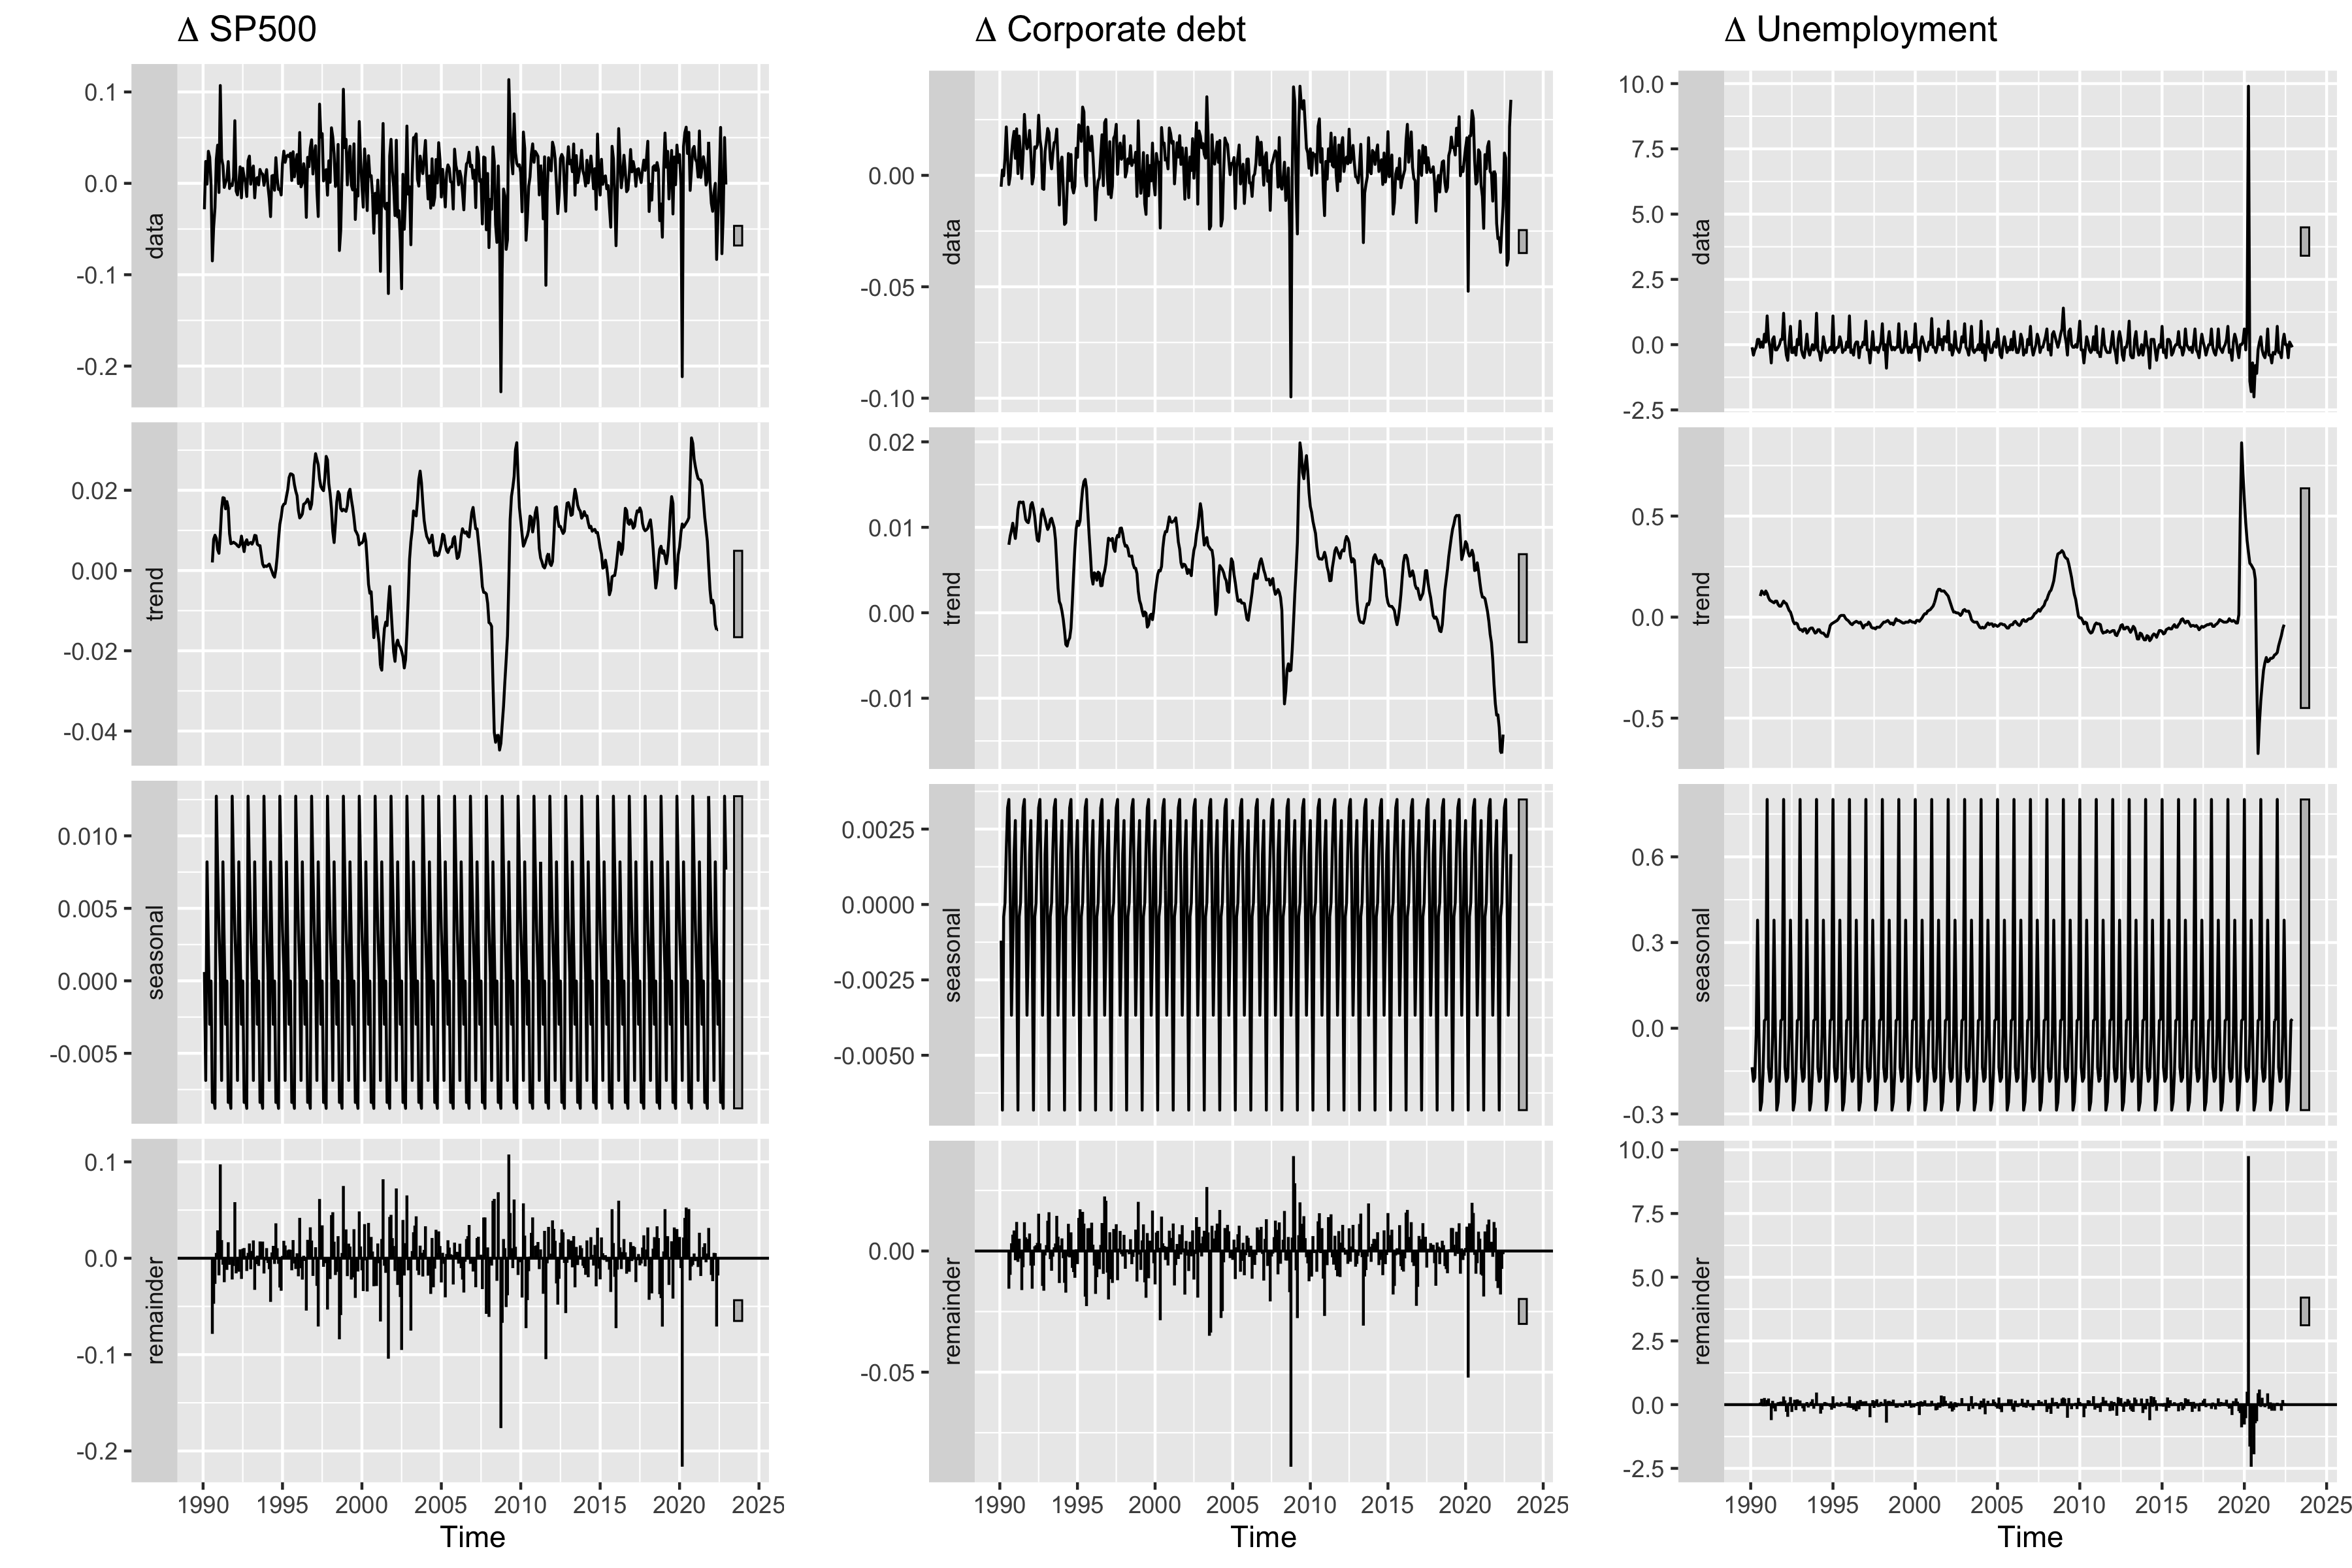
\includegraphics[width = 0.75\textwidth]{IMAGES/decomposition_iii_deltas.png}
    \caption{Decomposition of the series in deltas}
\end{figure}

    



    \subsection{Cyclical component}






\section{Canonical VAR model application}\label{sec:var}

% latex table generated in R 4.3.1 by xtable 1.8-4 package
% Tue Dec  5 14:47:20 2023
\begin{table}[ht]
\centering
\caption{Canonical VAR in levels - Identify order} 
\begin{tabular}{rrrrrrrrrrr}
  \hline
 & 1 & 2 & 3 & 4 & 5 & 6 & 7 & 8 & 9 & 10 \\ 
  \hline
AIC(n) & -10.01 & -10.56 & -10.59 & -10.73 & -10.88 & -10.87 & -10.93 & -11.01 & -11.00 & -10.98 \\ 
  HQ(n) & -9.96 & -10.48 & -10.47 & -10.57 & -10.68 & -10.64 & -10.66 & -10.71 & -10.66 & -10.60 \\ 
  SC(n) & -9.89 & -10.35 & -10.29 & -10.33 & -10.38 & -10.29 & -10.25 & -10.25 & -10.14 & -10.03 \\ 
  FPE(n) & 0.00 & 0.00 & 0.00 & 0.00 & 0.00 & 0.00 & 0.00 & 0.00 & 0.00 & 0.00 \\ 
   \hline
\end{tabular}
\end{table}



% Table created by stargazer v.5.2.3 by Marek Hlavac, Social Policy Institute. E-mail: marek.hlavac at gmail.com
% Date and time: Wed, Dec 13, 2023 - 20:23:41
\begin{table}[!htbp] \centering 
  \caption{Level VAR - Estimation} 
  \label{tab:est_var_level} 
\small 
\begin{tabular}{@{\extracolsep{5pt}}lccc} 
\\[-1.8ex]\hline 
\hline \\[-1.8ex] 
 & \multicolumn{3}{c}{\textit{Dependent variable:}} \\ 
\cline{2-4} 
\\[-1.8ex] & \multicolumn{3}{c}{y} \\ 
 & splong & rate & gdp \\ 
\hline \\[-1.8ex] 
 splong.l1 & 0.186$^{***}$ & 0.011$^{***}$ & 0.447$^{**}$ \\ 
  & (0.051) & (0.004) & (0.205) \\ 
  gdp.l1 & 3.065$^{***}$ & 0.912$^{***}$ & 17.259$^{***}$ \\ 
  & (0.664) & (0.051) & (2.646) \\ 
  rate.l1 & $-$0.037$^{***}$ & 0.001 & 0.442$^{***}$ \\ 
  & (0.013) & (0.001) & (0.052) \\ 
  splong.l2 & $-$0.101$^{*}$ & $-$0.011$^{***}$ & $-$0.410$^{**}$ \\ 
  & (0.052) & (0.004) & (0.207) \\ 
  gdp.l2 & $-$1.076 & $-$0.034 & $-$13.109$^{***}$ \\ 
  & (0.899) & (0.069) & (3.580) \\ 
  rate.l2 & $-$0.009 & $-$0.005$^{***}$ & 0.102$^{*}$ \\ 
  & (0.014) & (0.001) & (0.058) \\ 
  splong.l3 & 0.084 & 0.008$^{**}$ & 0.290 \\ 
  & (0.053) & (0.004) & (0.211) \\ 
  gdp.l3 & 0.359 & $-$0.712$^{***}$ & $-$2.540 \\ 
  & (0.920) & (0.071) & (3.663) \\ 
  rate.l3 & 0.030$^{**}$ & 0.004$^{***}$ & 0.210$^{***}$ \\ 
  & (0.015) & (0.001) & (0.059) \\ 
  splong.l4 & 0.017 & 0.005 & $-$0.131 \\ 
  & (0.054) & (0.004) & (0.214) \\ 
  gdp.l4 & $-$1.164 & 0.620$^{***}$ & 14.481$^{***}$ \\ 
  & (0.947) & (0.073) & (3.772) \\ 
  rate.l4 & 0.011 & 0.001 & $-$0.134$^{**}$ \\ 
  & (0.015) & (0.001) & (0.062) \\ 
  splong.l5 & 0.103$^{*}$ & $-$0.004 & $-$0.340 \\ 
  & (0.054) & (0.004) & (0.215) \\ 
  gdp.l5 & 0.896 & $-$0.075 & $-$7.278$^{**}$ \\ 
  & (0.900) & (0.070) & (3.583) \\ 
  rate.l5 & 0.026$^{*}$ & $-$0.001 & 0.009 \\ 
  & (0.016) & (0.001) & (0.062) \\ 
  splong.l6 & $-$0.174$^{***}$ & 0.011$^{***}$ & $-$0.028 \\ 
  & (0.054) & (0.004) & (0.215) \\ 
  gdp.l6 & $-$0.236 & $-$0.296$^{***}$ & $-$1.729 \\ 
  & (0.832) & (0.064) & (3.313) \\ 
  rate.l6 & $-$0.043$^{***}$ & 0.001 & 0.121$^{*}$ \\ 
  & (0.015) & (0.001) & (0.061) \\ 
  splong.l7 & 0.056 & $-$0.002 & $-$0.238 \\ 
  & (0.054) & (0.004) & (0.216) \\ 
  gdp.l7 & $-$0.645 & 0.216$^{***}$ & 3.930 \\ 
  & (0.639) & (0.049) & (2.543) \\ 
  rate.l7 & 0.039$^{***}$ & $-$0.001 & 0.006 \\ 
  & (0.014) & (0.001) & (0.056) \\ 
  const & 0.002 & 0.001$^{***}$ & $-$0.062$^{***}$ \\ 
  & (0.005) & (0.0004) & (0.021) \\ 
  trend & $-$0.00001 & $-$0.00000 & 0.0001$^{*}$ \\ 
  & (0.00002) & (0.00000) & (0.0001) \\ 
 \hline \\[-1.8ex] 
Adjusted R$^{2}$ & 0.145 & 0.626 & 0.488 \\ 
Residual Std. Error (df = 365) & 0.034 & 0.003 & 0.134 \\ 
F Statistic (df = 22; 365) & 3.991$^{***}$ & 30.486$^{***}$ & 17.760$^{***}$ \\ 
\hline 
\hline \\[-1.8ex] 
\textit{Note:}  & \multicolumn{3}{r}{$^{*}$p$<$0.1; $^{**}$p$<$0.05; $^{***}$p$<$0.01} \\ 
\end{tabular} 
\end{table} 


\section{Cointegration theory}\label{sec:cointegration}




\section{Impulse Response Analysis}\label{sec:irf}
    \subsection{Canonical IRF}\label{sec:canonical_irf}


    \subsection{Structural IRF}\label{sec:structural_irf}



\section{Introduce non-linearities}\label{sec:nonlinearities}
    \subsection{Markov-switching model}\label{sec:markov}

    
    \subsection{STR model}\label{sec:str}



\section{Difference-in-Difference}
https://www.tidy-finance.org/r/difference-in-differences.html
    
\end{document}